\subsection{Training Process}

\subsubsection{Training Settings}

Both models are trained for 100 epochs using pretrained YOLOv8 weights. Unless otherwise specified, the training process follows the default Ultralytics YOLOv8 settings. The batch size is set to 8, mixed-precision training (AMP) is enabled, and the optimizer is automatically selected as MuSGD with an initial learning rate of 0.01 and momentum 0.9. Early stopping with a patience of 50 epochs is also enabled. Mosaic augmentation is applied with probability 1.0 throughout most of the training process and is automatically disabled during the final 10 epochs following the default YOLOv8 training strategy. The learning rate schedule uses a warm-up stage during the first three epochs, after which the learning rate decreases linearly toward zero, as shown in Figure~\ref{fig:lr_schedule}.

\begin{figure}[h]
    \centering
    \includegraphics[width=0.5\textwidth]{figures/task2/LR schedule.png}
    \caption{Learning rate schedule during training.}
    \label{fig:lr_schedule}
\end{figure}

Figure~\ref{fig:training_batch} shows a representative augmented training batch containing 8 images. The visualization clearly demonstrates the effect of Mosaic augmentation, where multiple images are combined into a single training sample.

\begin{figure}[h]
    \centering
    \includegraphics[width=0.7\textwidth]{figures/task2/training batch.jpg}
    \caption{Visualization of an augmented training batch.}
    \label{fig:training_batch}
\end{figure}

\subsubsection{Training Dynamics Analysis}

Figure~\ref{fig:loss_curves} compares the Box Loss, Class Loss, and DFL Loss on both the training and validation sets. Overall, YOLOv8s-$768$ consistently achieves lower losses than YOLOv8n-$640$, indicating improved optimization and localization capability with the larger model capacity and higher input resolution.

For both models, the validation losses are initially lower than the training losses. This behavior is mainly caused by the strong data augmentation applied during training, which increases the difficulty of the training samples. During the final 10 epochs, disabling Mosaic augmentation causes a noticeable decrease in the training losses. In contrast, the validation losses remain relatively stable, indicating that the later-stage reduction in training loss mainly results from the removal of augmentation rather than a substantial improvement in generalization performance.

Among the three loss components, the largest improvement of YOLOv8s-$768$ appears in Box Loss and Class Loss, while the difference in DFL Loss is comparatively smaller. In particular, the validation DFL losses of the two models converge to nearly identical values at the end of training.

\begin{figure}[h]
    \centering
    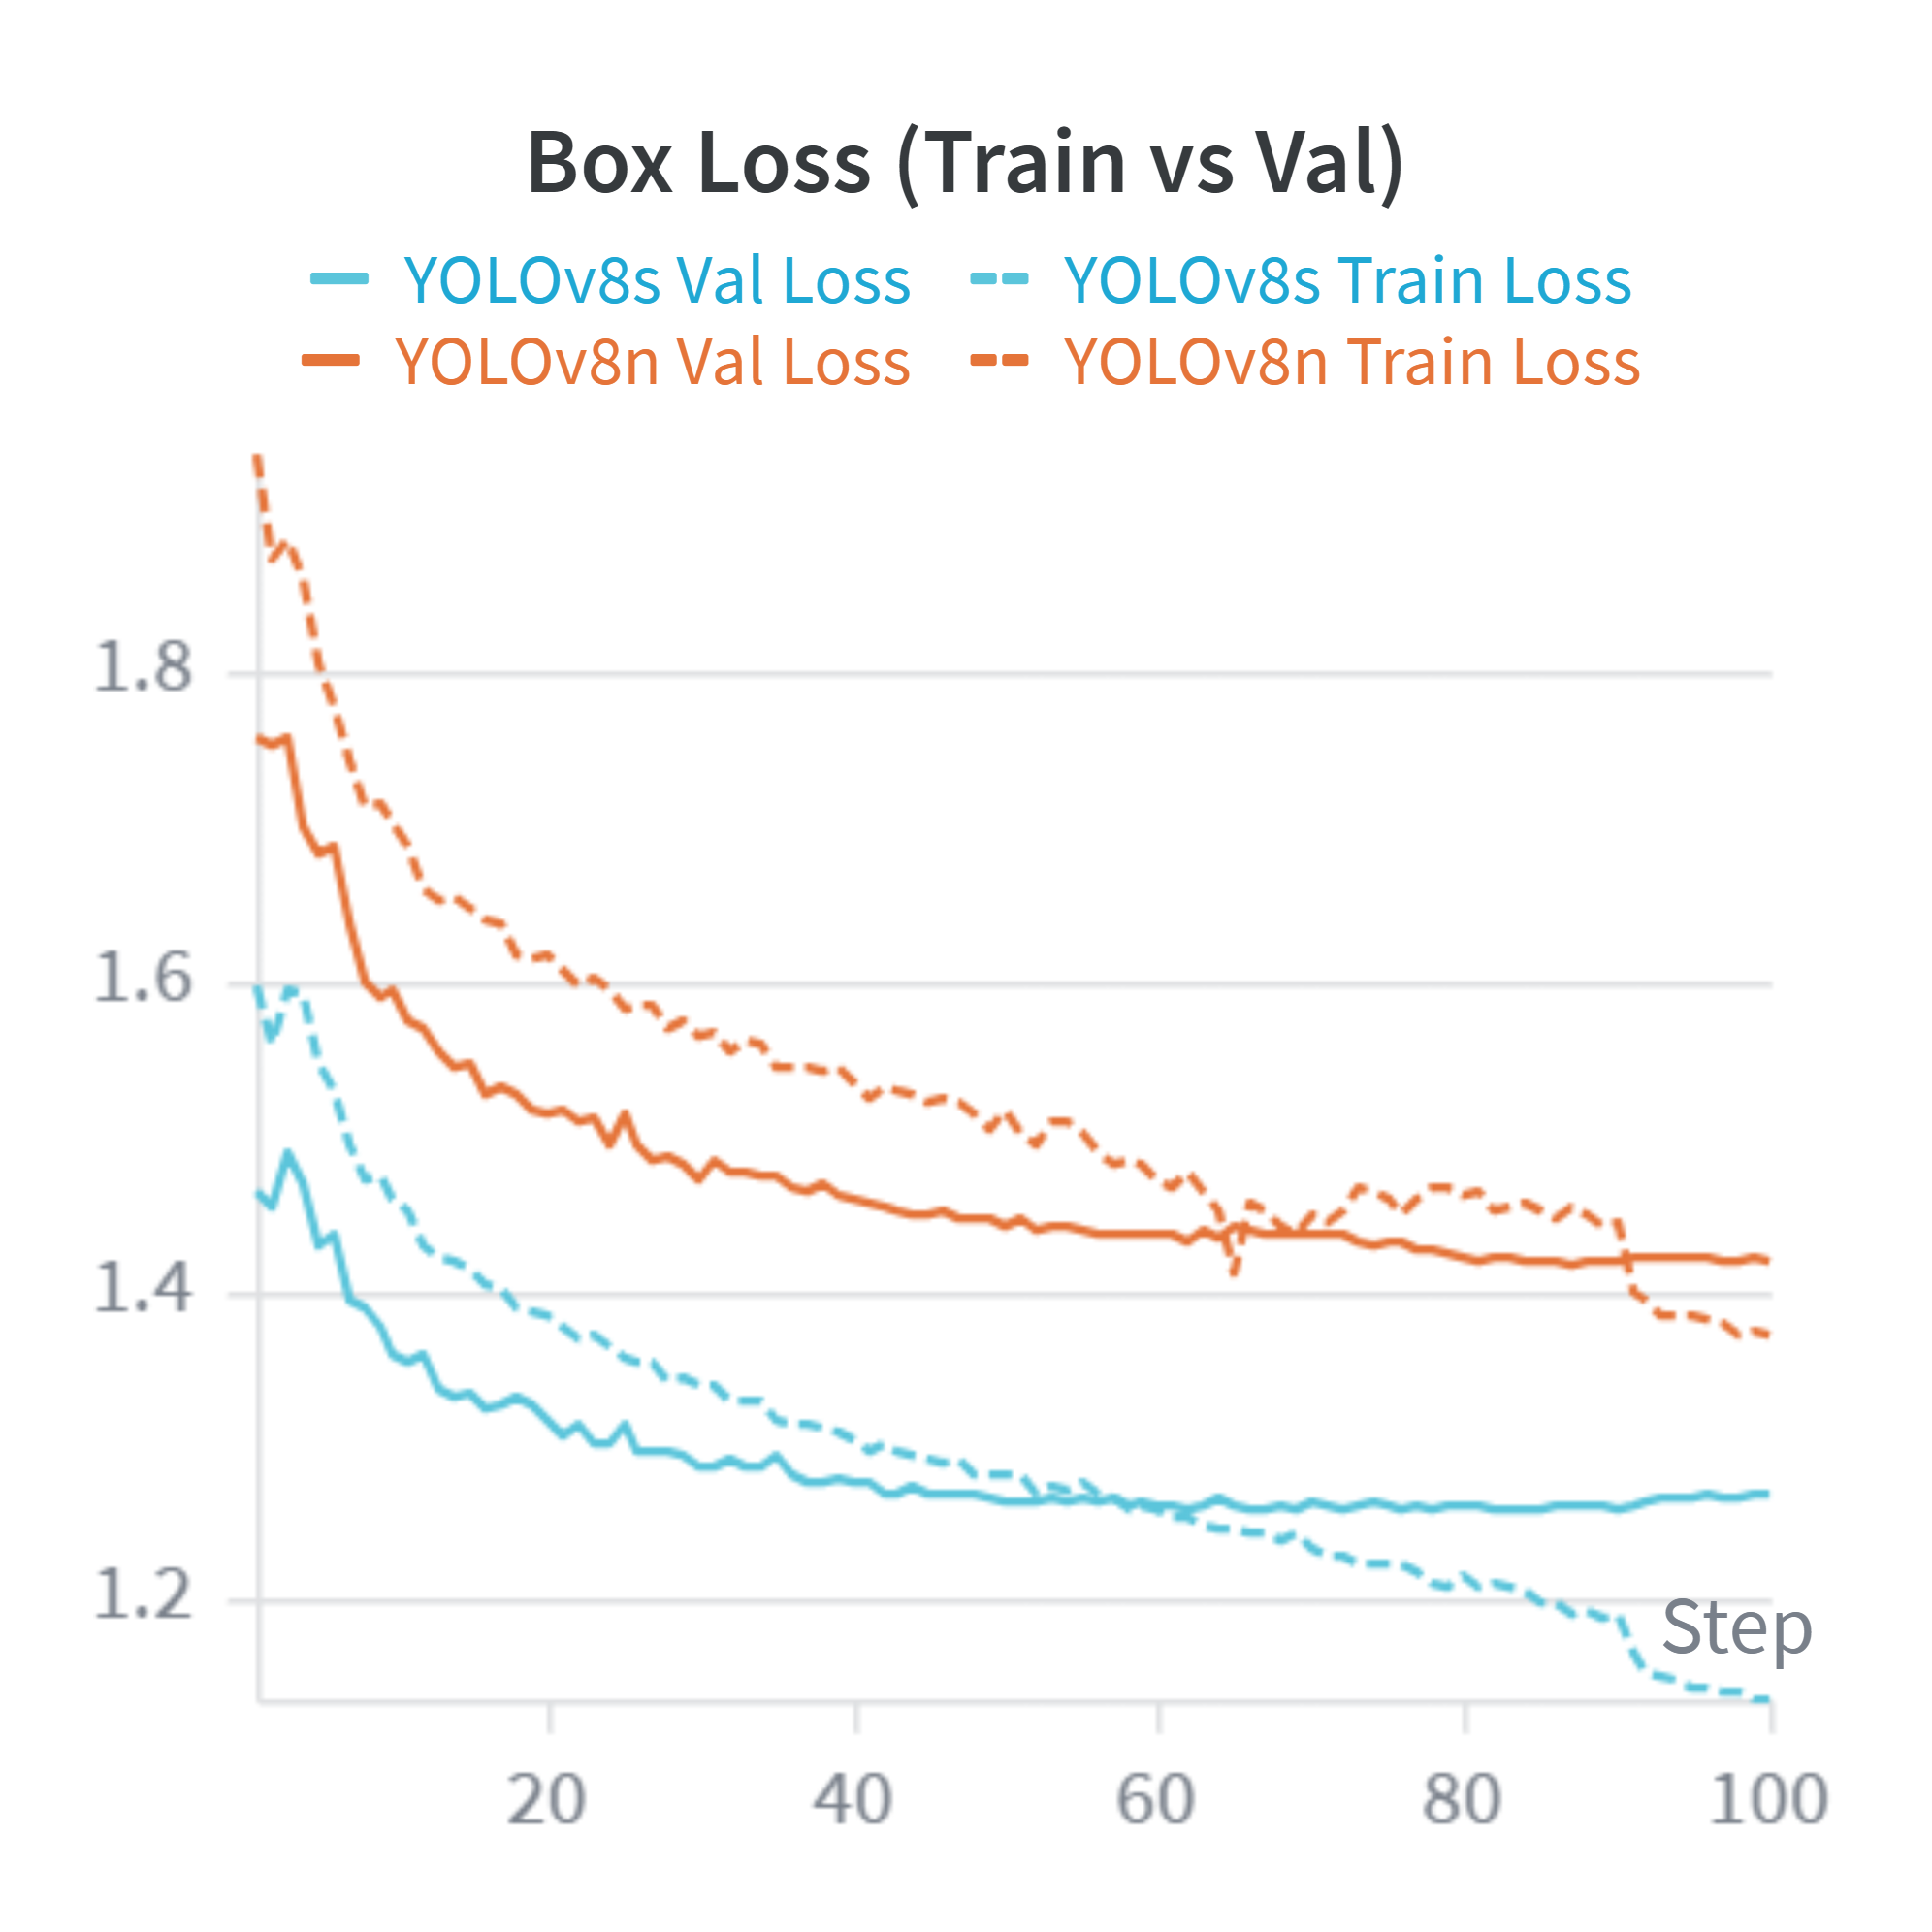
\includegraphics[width=0.32\textwidth]{figures/task2/Box Loss.png}
    \hfill
    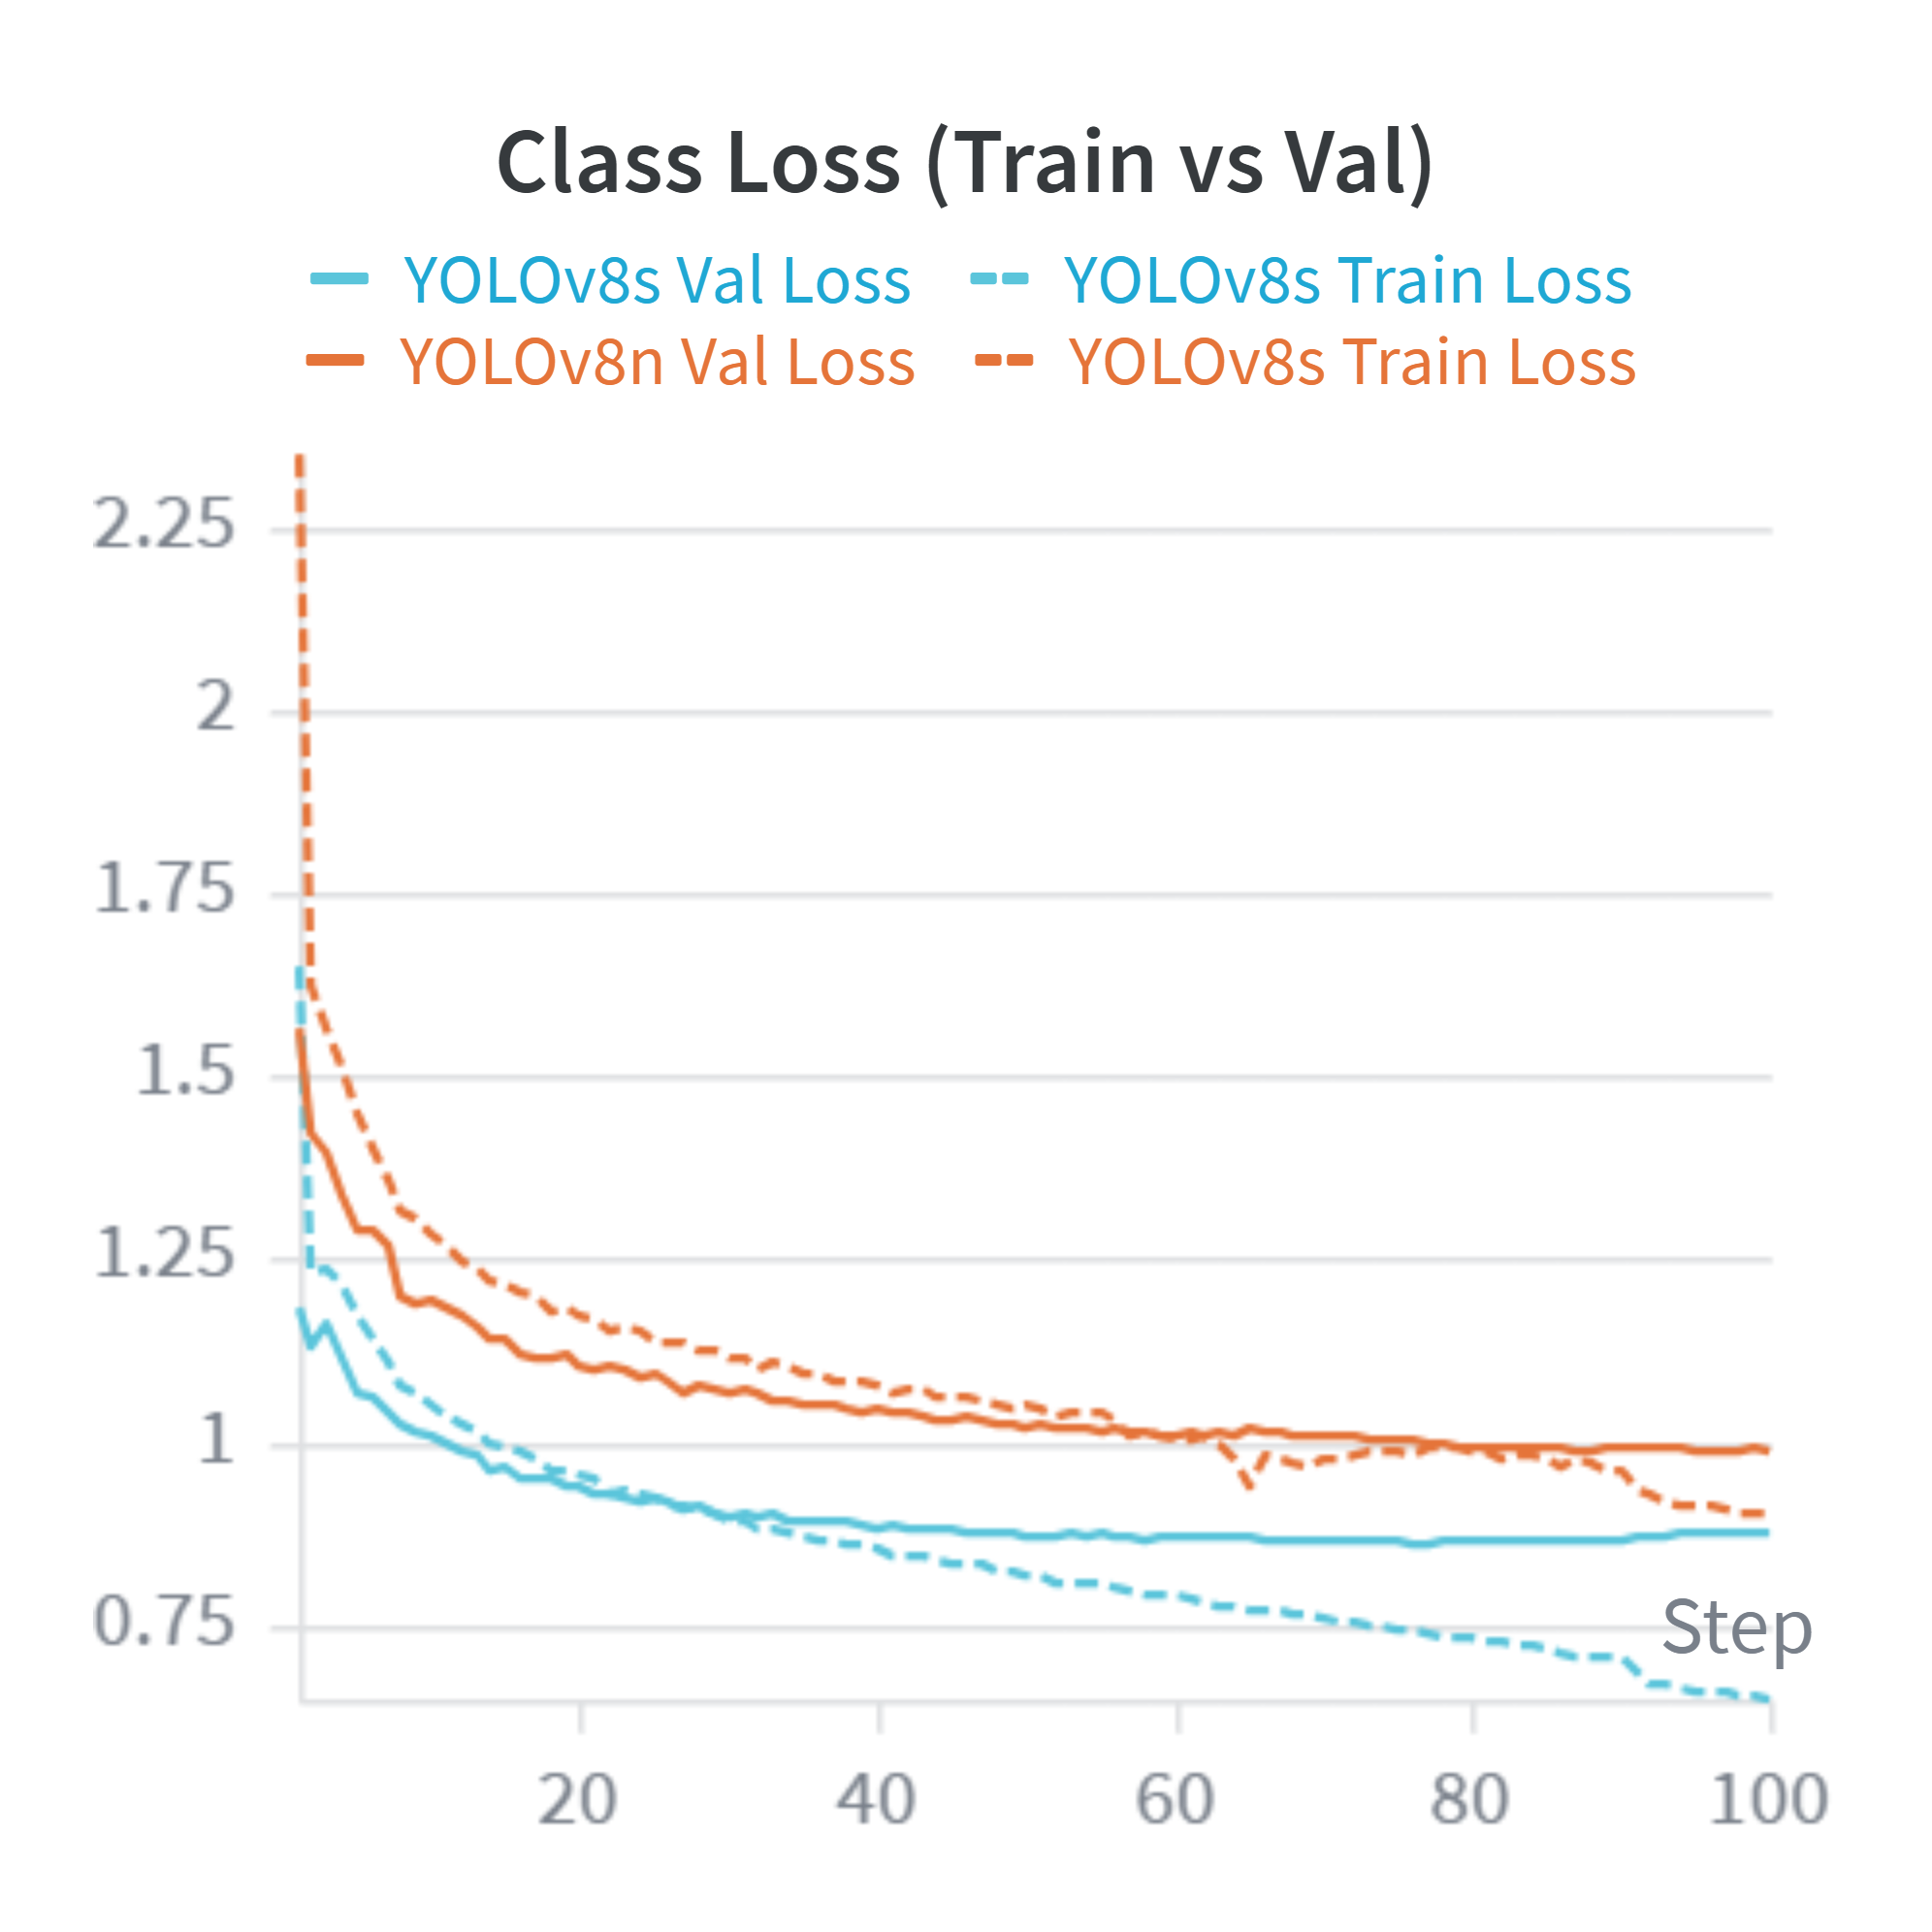
\includegraphics[width=0.32\textwidth]{figures/task2/Class Loss.png}
    \hfill
    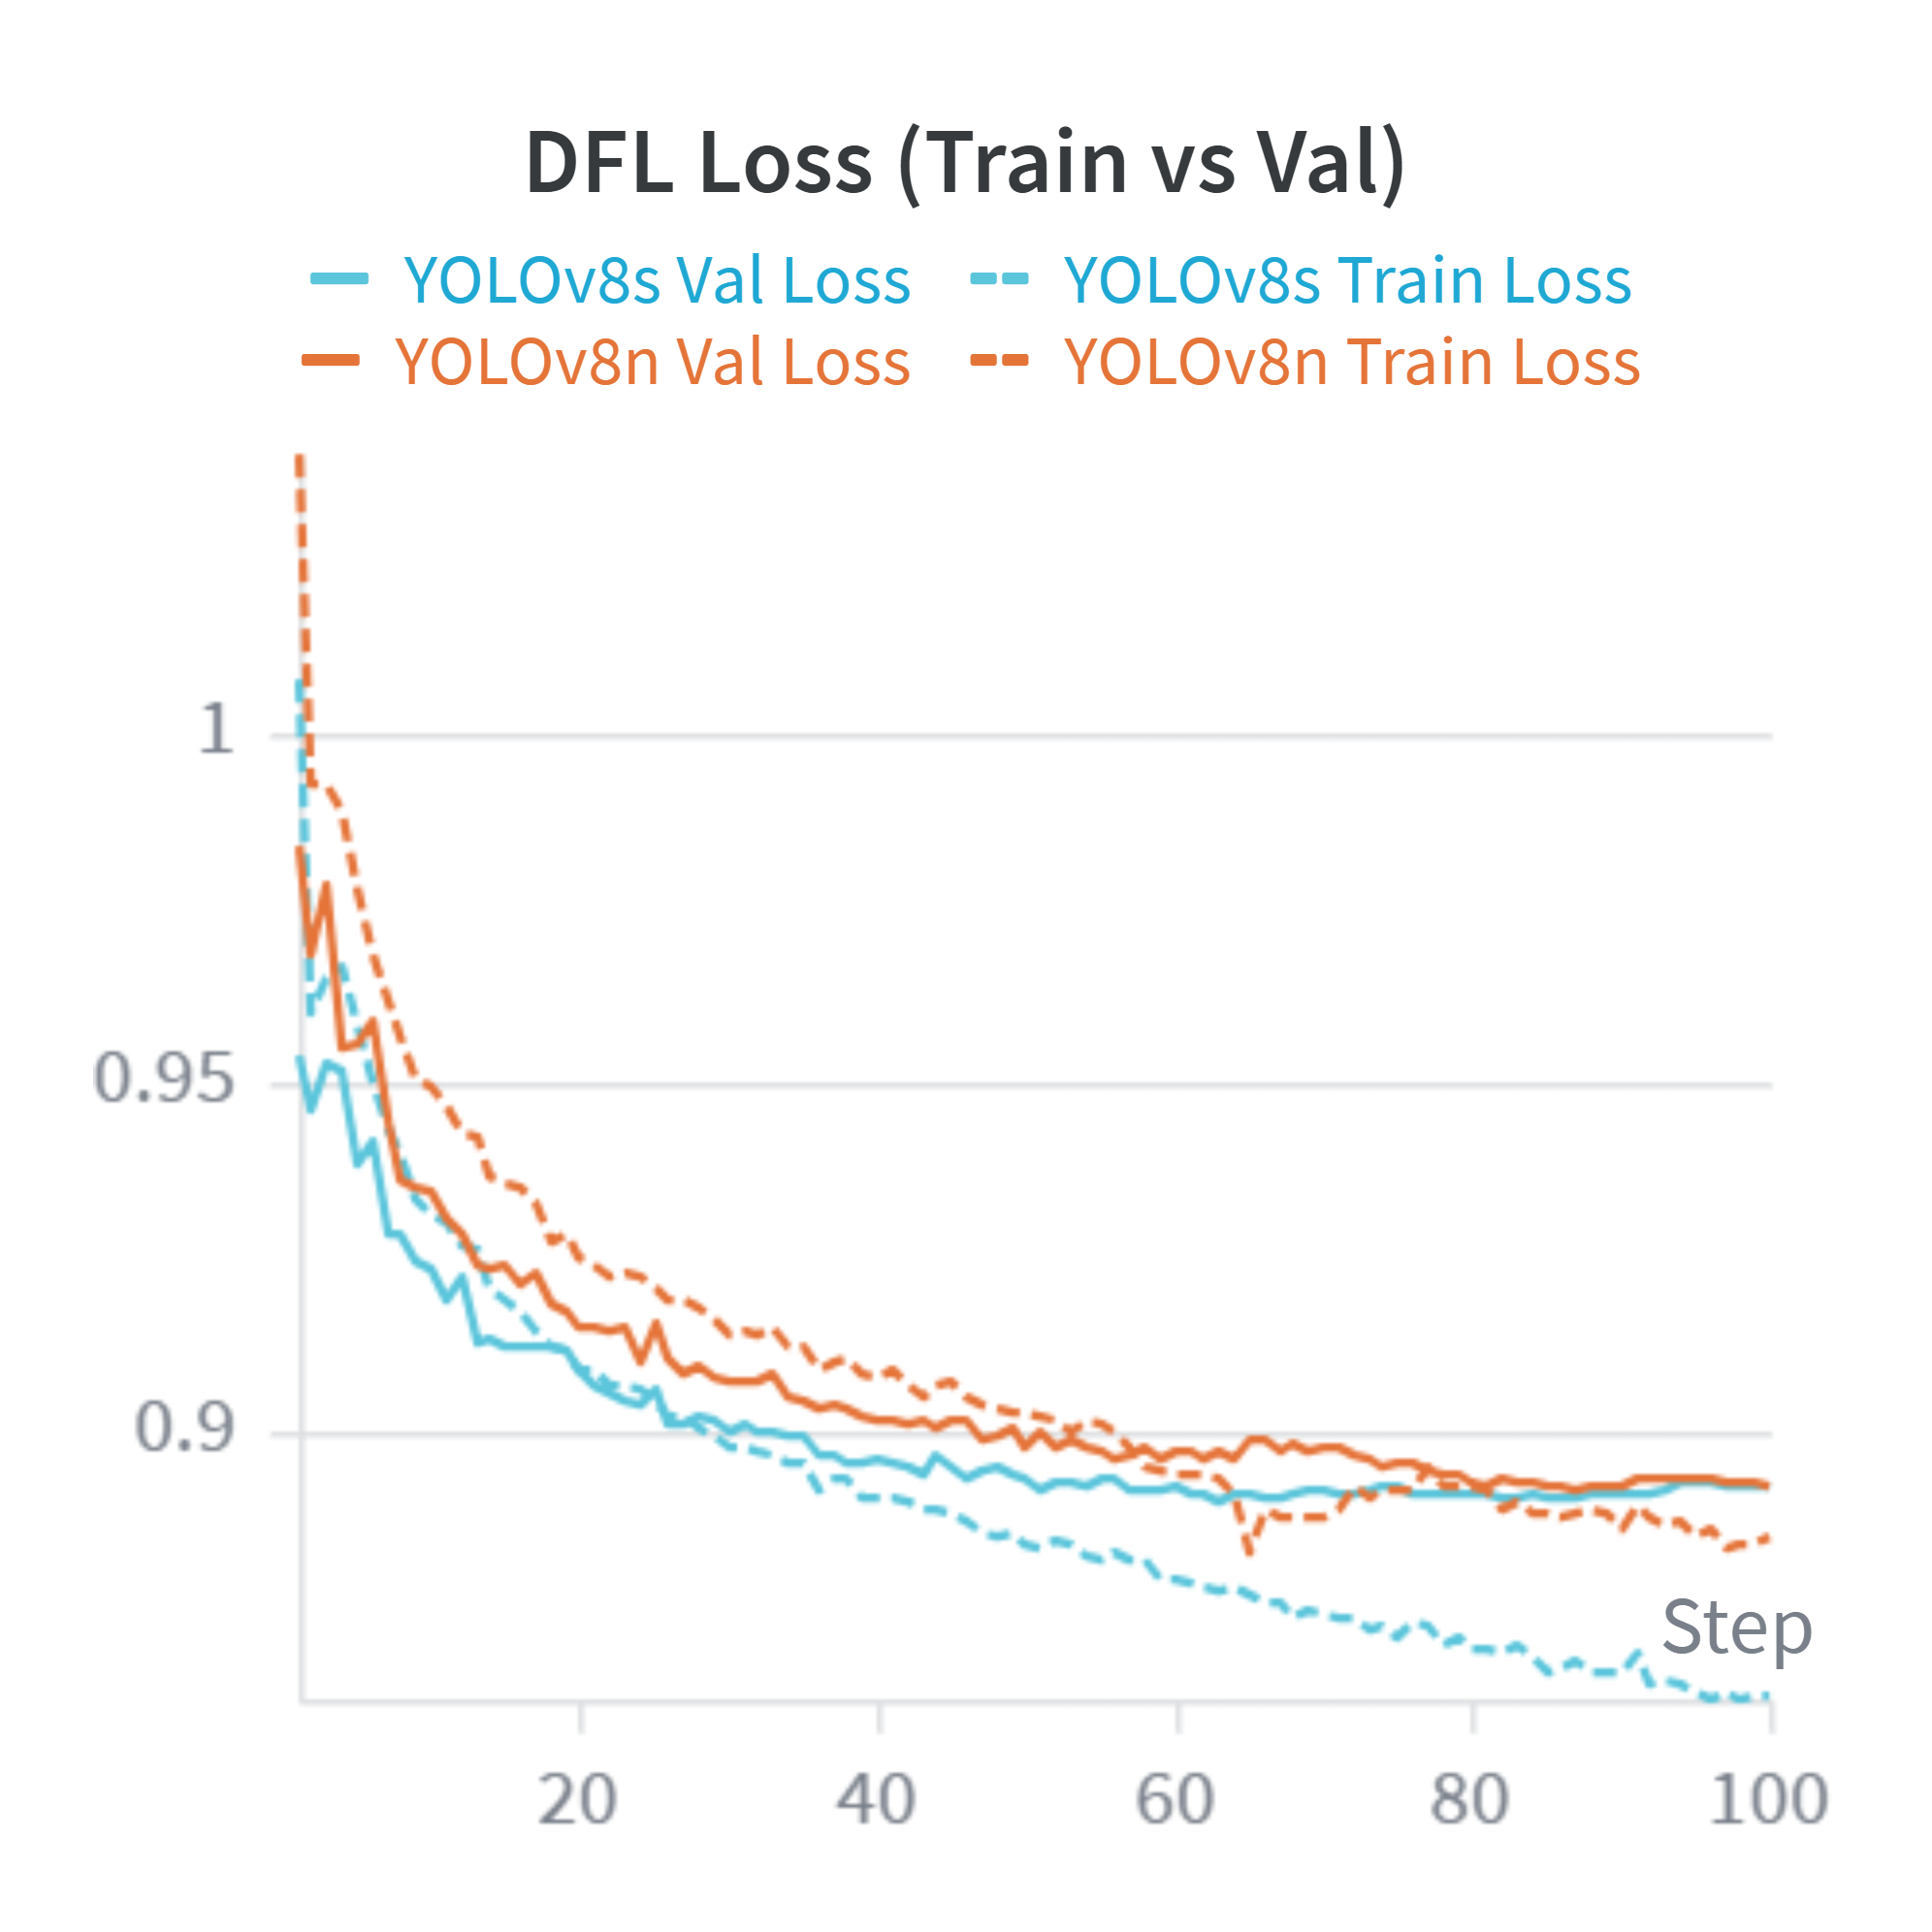
\includegraphics[width=0.32\textwidth]{figures/task2/DFL Loss.png}
    \caption{Comparison of Box Loss, Class Loss, and DFL Loss during training and validation.}
    \label{fig:loss_curves}
\end{figure}
